
\subsection{The construction of the grid $G_0$}\label{sec:construction-of-grids}

To construct the grid described in subsection \ref{sec:meshgrid} and Figure \ref{fig:gridex0},
we will use the number theory decomposition introduced by Victor Pambuccian in \cite{Pambuccian2016THEAO} and
Celia Schacht in \cite{Schacht2018ANOTHERAO}.

$$
n = \tau(n) \omega(n)
$$

where $\tau(n)$ is a power of 2 and $\omega(n)$ is an odd.

We can see directly from the Figure \ref{fig:gridex0} that the grid is constructed by the following rules:
\begin{itemize}
\item horizantal lines (blue, additional lines) satisfying $y = 2^k, k \in \mathbb{Z}$
\item vertical lines (green, multiplicative lines) satisfying
    \begin{itemize}
        \item the value of x satisfying $x = \frac{m}{2^l}, l \in \mathbb{Z}^+, m \in \mathbb{Z}$
        \item the assignment begin from $\omega(-m)$ and increase exponentially by power 2.
    \end{itemize}
\end{itemize}

\begin{figure}[ht]
\centering
\resizebox{0.9\textwidth}{!}{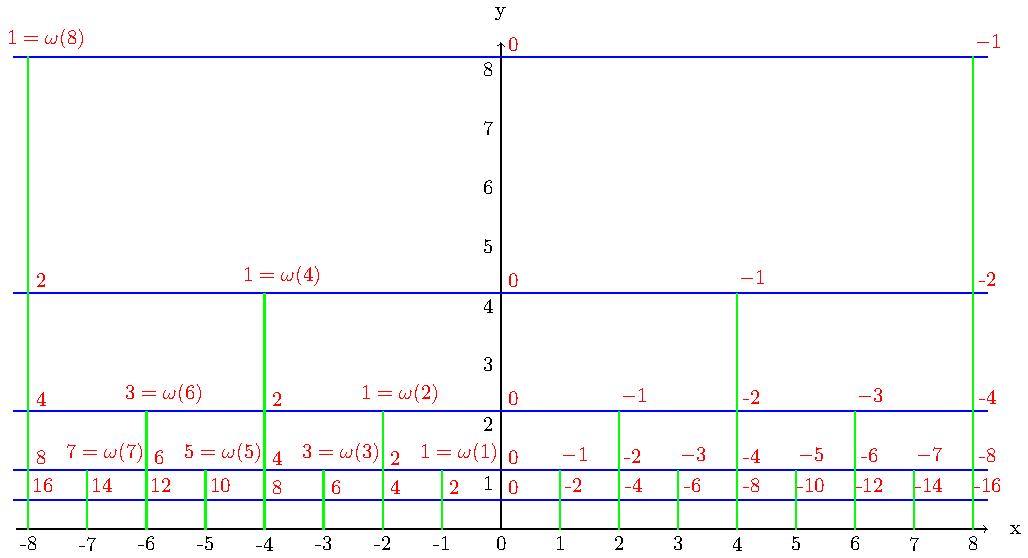
\includegraphics{images/07-grid-detail}}
\caption{$\omega$ gives the assignment at the start points of vertical lines in $G_0$}\label{fig:griddetail}
\end{figure}

The horizontal lines and the vertical lines divide the whole space into a mesh grid $G_0 = (V_0, E_0, F_0)$, where
$V_0$ is the set of crossing points, $E_0$ is the set of edges (segments in the horizontal and vertical lines,
it should be noted that only the vertical lines are geodesics, while the horizontal lines are horocycles) connecting
the crossing points, and $F_0$ is the set of cut cells. This mesh grid is generated by the additional generator $1$ and
the multiplicative generator $2$, and $V_0$, $E_0$, and $F_0$ are all countable sets.

We illustrate the construction schema of $G_0$ in Figure \ref{fig:gridschema}.

\begin{figure}[ht]
\centering
\resizebox{0.9\textwidth}{!}{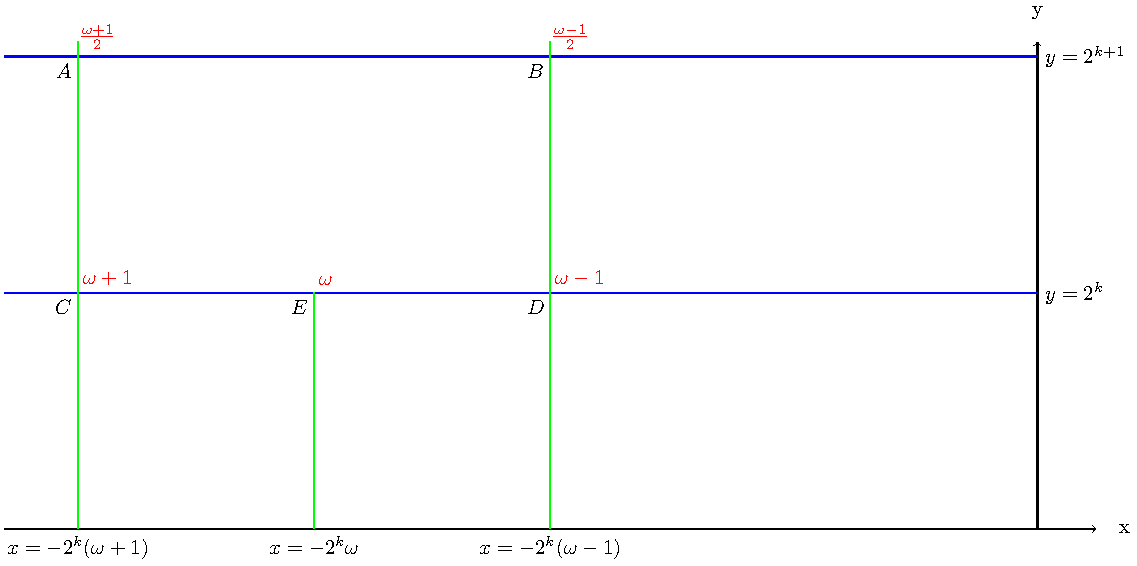
\includegraphics{images/08-grid-schema}}
\caption{the construction schema of $G_0$}\label{fig:gridschema}
\end{figure}

We notice that $G_0$ is very regular, in fact, all edges are equidistant.

\begin{lemma}\label{lem:regular}
All edges in $G_0$ are equidistant.
\end{lemma}

\begin{proof}
Following the construction schema in Figure \ref{fig:gridschema}, we can calculate the length of segments are all equidistant.

Length of $AC$ and $BD$:

$$
\int ds = \int\limits_{2^{k}}^{2^{k+1}} \frac{1}{y \ln 2} dy = \frac{1}{\ln 2} \left( \ln 2^{k+1} - \ln 2^k \right) = 1
$$

Length of $AB$:

$$
\int ds = \int\limits_{-2^k(\omega + 1)}^{-2^k(\omega - 1)} \frac{1}{2^{k+1}} dx = \frac{1}{2^{k+1}} \left( 2^{k + 1} \right) = 1
$$

Length of $CE$:

$$
\int ds = \int\limits_{-2^k(\omega + 1)}^{-2^k \omega} \frac{1}{2^k} dx = \frac{1}{2^k} \left( 2^k \right) = 1
$$

Length of $ED$:

$$
\int ds = \int\limits_{-2^k \omega}^{-2^k(\omega - 1)} \frac{1}{2^k} dx = \frac{1}{2^k} \left( 2^k \right) = 1
$$
\end{proof}

\subsection{The construction of the grid $G_1$}\label{sec:construction-of-grids}

We can similarly construct the grid $G_1$ using the additional generator $\frac{1}{2}$ and the multiplicative generator
$\sqrt{2}$, the grid $G_2$ using the additional generator $\frac{1}{4}$ and the multiplicative generator $\sqrt[4]{2}$,
and so on. And each time the cell of the mesh grid is divided into smaller cells and the end points of the vertical lines
move upward.

\begin{figure}[ht]
\centering
\resizebox{0.9\textwidth}{!}{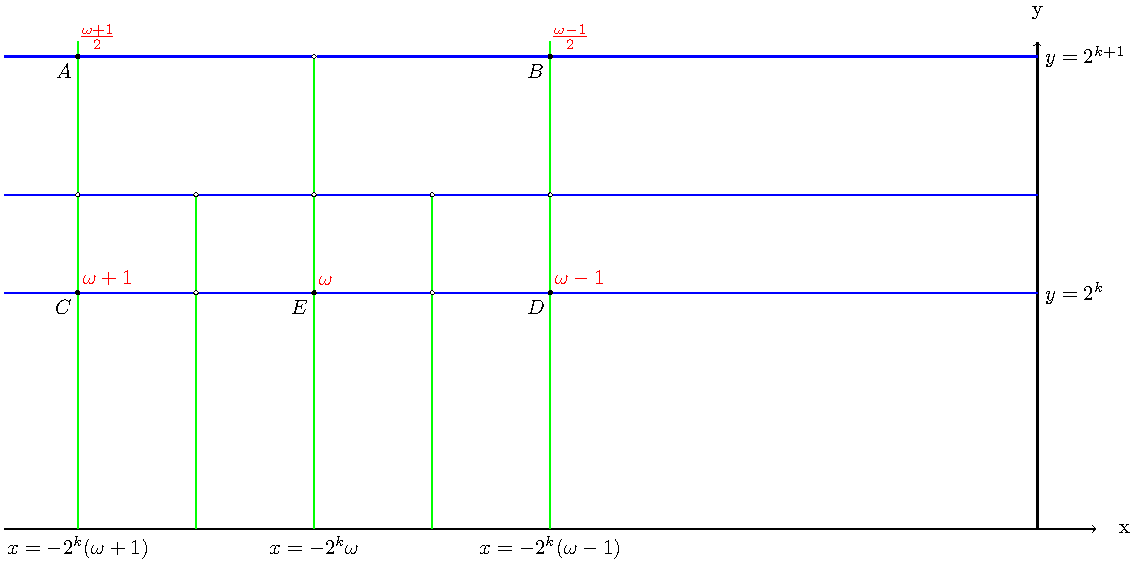
\includegraphics{images/09-grid-schema-g1}}
\caption{the construction schema of $G_1$}\label{fig:gridschemag1}
\end{figure}

\subsection{The construction of the grid $G_2$}\label{sec:construction-of-grids}


\subsection{The grid mesh is dense}\label{sec:construction-of-grids}

It is easy to see that there is a chain of inclusion relations:
$$
V_0 \subset V_1 \subset V_2 \subset \cdots V_i \subset \cdots
$$

Suppose $V = \bigcup_{i=1}^{\infty} V_i$, we have below lemma

\begin{lemma}
$V$ is a countable dense set.
\end{lemma}

\begin{proof}
Because $V_i$ is countable, and the union is over a countable index set, so $V$ is countable.

We can prove it is dense by contradiction. Suppose $V$ is not a dense set. Then there is a point $p$ in the space
neither belongs to $V$ nor is a limit point of $V$.

TODO...

\end{proof}

\subsection{Completeness and topology}\label{sec:topdef}

\subsection{As a special integral}\label{sec:integral}

\newpage
